\chapter{}

In Section \ref{sec:solving_YM}, a way to calculate the chromodynamic fields in the forward light-cone as a function of the pre-collision potentials was provided (Eqs. (\ref{eq:chromodynamic_fields_full})). Chapter \ref{sec:Margaret}, in turn, showed how to extract, from the chromodynamic fields, values for the stopping power and for the momentum broadening coefficient (Eqs. (\ref{eq:collision_from_tensors})), quantities which characterize the pre-hydrodynamic stage "macroscopically". The present chapter will be concerned with the insertion of the results of Section \ref{sec:solving_YM} into the machinery of Chapter \ref{sec:Margaret}, and the simplification of the resulting expressions.

\section{Handling the $X^{\alpha \beta}$ tensor}
\subsection{Calculating components of $X^{\alpha \beta}$ }

In order to  calculate the components of the $X^{\alpha \beta}$ tensor, the chromodynamic field expressions of Eqs. (\ref{eq:chromodynamic_fields_full}) are plugged into Eq. (\ref{eq:unfolded_X}). This can be made easier by remembering the shared structure of the chromodynamic field expressions detailed in Eq. (\ref{eq:shared_structure}). Any two-point correlator of chromodynamic fields may thus be written as:
\begin{equation}
\label{eq:generalized_chromodynamic_correlator}
\begin{alignedat}{1}
\Big< {G_1^\alpha}_a  (t,\mathbf{x}) {G_2^\beta}_a (t',\mathbf{y}) \Big>
 = & \Bigg<\int  \frac{\diff^2 \mathbf{k_\perp}}{(2\pi)^2}
\int \frac{\diff^2 \mathbf{l}_\perp}{(2\pi)^2}
\int \diff^2  \mathbf{u}_\perp 
\int \diff^2 \mathbf{w}_\perp 
\left[ C_1^{ij} C_2^{mn}
D^\alpha (\tau, \mathbf{x}_\perp) D^\beta (\tau', \mathbf{y}_\perp)  \right] \\
&  e^{i \mathbf{k}_\perp \cdot (\mathbf{x} - \mathbf{u})_\perp}
e^{i \mathbf{l}_\perp \cdot (\mathbf{y} - \mathbf{w})_\perp}
f^{bca} f^{dea}
 \alpha^i_{1b} (\mathbf{u}_\perp) \alpha^j_{2c} (\mathbf{u}_\perp) \alpha^m_{1d} (\mathbf{w}_\perp)   \alpha^n_{2e} (\mathbf{w}_\perp) \Bigg> \\
  = & \int  \frac{\diff^2 \mathbf{k_\perp}}{(2\pi)^2}
\int \frac{\diff^2 \mathbf{l}_\perp}{(2\pi)^2}
\int \diff^2 \mathbf{u}_\perp
 \int \diff^2 \mathbf{w}_\perp 
\left[ C_1^{ij} C_2^{mn}
D^\alpha (\tau, \mathbf{x}_\perp) D^\beta (\tau', \mathbf{y}_\perp)  \right] \\
&  e^{i \mathbf{k}_\perp \cdot (\mathbf{x} - \mathbf{u})_\perp}
e^{i \mathbf{l}_\perp \cdot (\mathbf{y} - \mathbf{w})_\perp}
 f^{bca} f^{dea}
 \big< \alpha^i_{1b} (\mathbf{u}_\perp) \alpha^m_{1d} (\mathbf{w}_\perp) \big>
 \big< \alpha^j_{2c} (\mathbf{u}_\perp) \alpha^n_{2e} (\mathbf{w}_\perp) \big>
\end{alignedat}
\end{equation}
where $\tau$ and $\tau'$ are obtained from cartesian coordinates as usual: $\tau = \sqrt{t^2 - \mathbf{x}^2}$, $\tau' = \sqrt{t'^2 - \mathbf{y}^2}$. At the second equality, the gluon fields have been paired up in two-point correlators, as gluon fields from different incoming nuclei are uncorrelated, due to them being causally unrelated.

Given that, between different correlators, only the terms in square brackets change, one may concentrate on them when calculating the $X^{\alpha \beta}$ tensor components by following Eq. (\ref{eq:unfolded_X}). This allows postponing concern with the integrals and the color space section of Eq. (\ref{eq:generalized_chromodynamic_correlator}). All of the components are treated in this manner and the simplified results are shown in Appendix \ref{X_components}.

\subsection{Calculating projections of $X^{\alpha \beta}$}

The components of the $X^{\alpha \beta}$ tensor must now be used to calculate the projections needed to calculate $\hat{q}$ and $\diff E / \diff x$ (Eq. (\ref{eq:collision_from_tensors})). These projections can be simplified into a surprisingly compact form, considering the amount of terms involved in each of them:
\begin{subequations}
\begin{alignat}{2}
\begin{split}
v^\alpha v^\beta X^{\alpha \beta} = \int & \frac{\diff^2 \mathbf{k_\perp}}{(2\pi)^2}
\int \frac{\diff^2 \mathbf{l}_\perp}{(2\pi)^2}
\int \diff^2 \mathbf{u}_\perp
 \int \diff^2 \mathbf{w}_\perp  
\\
& \left[ (v^1)^2 J_0 (k \tau) J_0(l\tau') \delta^{ij} \delta^{mn} - \left(\frac{\mathbf{v}_\perp \times \mathbf{k}_\perp}{k}\frac{\mathbf{v}_\perp \times \mathbf{l}_\perp}{l}\right) J_1 (k \tau) J_1(l\tau') \varepsilon^{ij} \varepsilon^{mn} \right]
\\
& e^{i \mathbf{k}_\perp \cdot (\mathbf{x} - \mathbf{u})_\perp}
e^{i \mathbf{l}_\perp \cdot (\mathbf{y} - \mathbf{w})_\perp}
f^{bca} f^{dea}
 \big< \alpha^i_{1b} (\mathbf{u}_\perp) \alpha^m_{1d} (\mathbf{w}_\perp) \big>
 \big< \alpha^j_{2c} (\mathbf{u}_\perp) \alpha^n_{2e} (\mathbf{w}_\perp) \big>
\end{split} \\
\begin{split}
\delta^{\alpha \beta} X^{\alpha \beta} = \int & \frac{\diff^2 \mathbf{k_\perp}}{(2\pi)^2}
\int \frac{\diff^2 \mathbf{l}_\perp}{(2\pi)^2}
\int \diff^2 \mathbf{u}_\perp
 \int \diff^2 \mathbf{w}_\perp  
 \\
 & \Bigg[ (\delta^{ij} \delta^{mn} + {v_\perp}^2 \varepsilon^{ij} \varepsilon^{mn}) J_0 (k \tau) J_0(l\tau') + i \frac{\mathbf{v}_\perp \cdot \mathbf{l}_\perp}{l} (\delta^{ij} \delta^{mn} - \varepsilon^{ij} \varepsilon^{mn}) J_0 (k \tau) J_1(l\tau') \\
&  + i \frac{\mathbf{v}_\perp \cdot \mathbf{k}_\perp}{k} (\delta^{ij} \delta^{mn} - \varepsilon^{ij} \varepsilon^{mn}) J_1 (k \tau) J_0(l\tau')  \\
& - \bigg( \Big(\frac{\mathbf{v}_\perp \cdot \mathbf{k}_\perp}{k} \frac{\mathbf{v}_\perp \cdot \mathbf{l}_\perp}{l} + (v^1)^2 \frac{\mathbf{k}_\perp \cdot \mathbf{l}_\perp}{k~l} \Big) \delta^{ij} \delta^{mn} + \frac{\mathbf{k}_\perp \cdot \mathbf{l}_\perp}{k ~l} \varepsilon^{ij}\varepsilon^{mn} \bigg) J_1 (k \tau) J_1\big(l\tau'\big) \Bigg]
 \\
& e^{i \mathbf{k}_\perp \cdot (\mathbf{x} - \mathbf{u})_\perp}
e^{i \mathbf{l}_\perp \cdot (\mathbf{y} - \mathbf{w})_\perp}
f^{bca} f^{dea}
 \big< \alpha^i_{1b} (\mathbf{u}_\perp) \alpha^m_{1d} (\mathbf{w}_\perp) \big>
 \big< \alpha^j_{2c} (\mathbf{u}_\perp) \alpha^n_{2e} (\mathbf{w}_\perp) \big>
\end{split}
\end{alignat}
\label{eq:unintegrated_X_projections}
\end{subequations}
where $\mathbf{a}_\perp \times \mathbf{b}_\perp$ is the 2-dimensional cross product. It is defined as $\mathbf{a}_\perp \times \mathbf{b}_\perp \equiv \varepsilon^{ij} {a_\perp}^i {b_\perp}^j = |\mathbf{a}_\perp| |\mathbf{b}_\perp| \sin \hat{\left(\mathbf{a}_\perp,\mathbf{b}_\perp \right)} $; particularly, $\left( \mathbf{a}_\perp \times \mathbf{b}_\perp \right) \left( \mathbf{a}_\perp \times \mathbf{c}_\perp \right) = {\mathbf{a}_\perp}^2 \left(\mathbf{b}_\perp \cdot \mathbf{c}_\perp \right) - \left(\mathbf{a}_\perp \cdot \mathbf{b}_\perp \right) \left(\mathbf{a}_\perp \cdot \mathbf{c}_\perp \right)$.

The next step is to compute the integrals analytically to the greatest extent possible.

\subsection{Computing the integrals}

Similar techniques to those employed in \cite{Guerrero_Rodr_guez_2021} will be used to simplify Eqs. (\ref{eq:unintegrated_X_projections}). First, the order of integration of the Fourier and inverse Fourier transforms is swapped, and the latter are converted to polar coordinates. As before, $k$ and $l$ denote the Euclidean norms of $\mathbf{k}_\perp$ and $\mathbf{l}_\perp$; additionally,
\begin{subequations}
\begin{align}
k^2 & \equiv k \cos \theta_k \\
k^3 & \equiv k \sin \theta_k
\end{align}
\end{subequations}
and similarly for $\mathbf{l}_\perp$ with the definition of $\theta_l$. The angular variables are defined such that $\theta_k$ measures the angle between $(\mathbf{x}-\mathbf{u})_\perp$ and $\mathbf{k}_\perp$, and $\theta_l$ measures the angle between $(\mathbf{y}-\mathbf{w})_\perp$ and $\mathbf{l}_\perp$, as illustrated in Fig. \ref{fig:angles}. Due to the change of variables,
\begin{subequations}
\begin{align}
	\int \frac{\diff^2 \mathbf{k_\perp}}{(2\pi)^2}
\int \frac{\diff^2 \mathbf{l}_\perp}{(2\pi)^2} \quad & \to
\quad \int_0^{+\infty} \frac{\diff k}{2\pi} k
\int_0^{+\infty} \frac{\diff l}{2\pi} l
\int_{0}^{2\pi} \frac{\diff \theta_k}{2 \pi} \int_{0}^{2\pi} \frac{\diff \theta_l}{2 \pi} \\
e^{i \mathbf{k}_\perp \cdot (\mathbf{x} - \mathbf{u})_\perp}
e^{i \mathbf{l}_\perp \cdot (\mathbf{y} - \mathbf{w})_\perp} \quad &\to \quad 
e^{i k |\mathbf{x}_\perp - \mathbf{u}_\perp| \cos{\theta_k}}
e^{i l |\mathbf{y}_\perp - \mathbf{w}_\perp| \cos{\theta_l}}\\
(\mathbf{v}_\perp \times \mathbf{k}_\perp) (\mathbf{v}_\perp \times \mathbf{l}_\perp) \quad & \to \quad \\
\mathbf{v}_\perp \cdot \mathbf{q}_\perp  \quad & \to \quad \\
(\mathbf{v}_\perp \cdot \mathbf{k}_\perp) (\mathbf{v}_\perp \cdot \mathbf{l}_\perp)  \quad & \to \quad \\
\mathbf{k}_\perp \cdot \mathbf{l}_\perp  \quad & \to \quad 
k l \cos \left( \theta_{y-w} + \theta_l - \left(\theta_{x-u} + \theta_k \right) \right)
\end{align}
\end{subequations}


\begin{figure}
    \centering
    %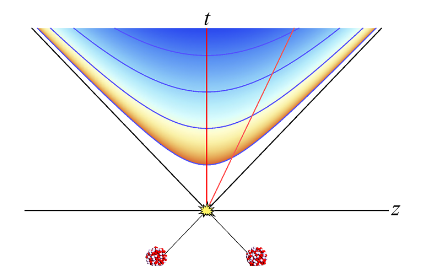
\includegraphics[width=0.7\textwidth]{Figures/HIC_lightcone.png} %PLACEHOLDER
    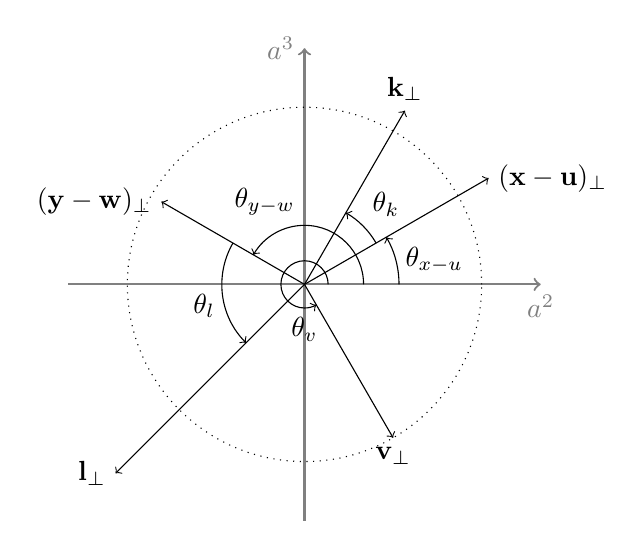
\begin{tikzpicture}[scale=1.5]
%axes
\draw[->,gray,thick] (-2,0) -- (2,0) node[below] {$a^2$};
\draw[->,gray,thick] (0,-2) -- (0,2) node[left] {$a^3$}; 
%circle
\draw[color = black,dotted] (0,0) circle (1.5);
%vectors
\draw[->] (0,0) -- (1.559,0.9) node[right] {$(\mathbf{x}-\mathbf{u})_\perp$};
\draw[->] (0,0) -- (0.85,1.472) node[above] {$\mathbf{k}_\perp$};
\draw[->] (0,0) -- (-1.212,0.7) node[left] {$(\mathbf{y}-\mathbf{w})_\perp$};
\draw[->] (0,0) -- (-1.6,-1.6) node[left] {$\mathbf{l}_\perp$};
\draw[->] (0,0) -- (0.75,-1.299) node[below] {$\mathbf{v}_\perp$};

%arcs
\draw[->] (0.8,0) arc [start angle=0, end angle=30, radius=0.8] node[pos=0.5, right] {$\theta_{x-u}$};
\draw[->] (0.5,0) arc [start angle=0, end angle=150, radius=0.5] node[pos=0.6, above left] {$\theta_{y-w}$};
\draw[->] (0.2,0) arc [start angle=0, end angle=300, radius=0.2] node[pos=0.9, below] {$\theta_v$};
\draw[->] (0.606,0.35) arc [start angle=30, end angle=60, radius=0.7] node[pos=0.5, above right] {$\theta_k$};
%\node at (0.7,0.7) {$\theta_k$};
\draw[->] (-0.606,0.35) arc [start angle=150, end angle=225, radius=0.7] node[pos=0.6, left] {$\theta_l$};
%\node at (-0.7,-0.2) {$\theta_l$};
\end{tikzpicture}
    \caption{Relative positions and angles defined between the vectors $(\mathbf{x}-\mathbf{u})_\perp$, $(\mathbf{y}-\mathbf{w})_\perp$, $\mathbf{k}_\perp$, $\mathbf{l}_\perp$ and $\mathbf{v}_\perp$ at some point in the integration.}
    \label{fig:angles}
\end{figure}




